\chapter{\label{ch:ch4} Design ad Implementation}

This chapter outlines the design and implementation phases of the mobile robot system project. The purpose of this chapter is to describe the system’s architecture, the design of each subsystem, the integration of hardware and software, and how these components work together to achieve the goals of this project. The design emphasizes ease of navigation, real-time feedback, and effective control via an intuitive interface.

\section{\label{sec:ch4_firstsec}System Design}

The design of the mobile robot system was based on the specific project requirements outlined in Chapter\ref{ch:req_and_specs}. Following a detailed review of relevant literature and an analysis of system needs, the robot’s overall design was established. The architecture integrates several key components—Raspberry Pi, camera module, fiducial markers, motor control system, and wireless communication modules—to ensure optimal system performance.

The core decision-making process involved selecting the appropriate technologies and components. Based on the findings from previous research (e.g., Jacobsen et al. \cite{jacobsen2018}, La Delfa et al. \cite{delfa2015}, and Vanitha et al. \cite{vanitha2016}), which explored various mobile robot control methods using augmented reality (AR) and computer vision, it became clear that a Raspberry Pi-based system with a web interface would provide the required flexibility and ease of control for this project.

After evaluating several options for actuation and navigation, it was determined that motorized control through a motor driver and a four-wheel drive system would provide the most reliable and efficient solution for movement. This decision was supported by studies that demonstrate the performance of motor-driven robots in both laboratory and dynamic environments. Additionally, the use of fiducial markers, such as ArUco or AprilTag markers, was identified as a robust solution for localization and obstacle avoidance (La Delfa et al. \cite{delfa2015}; Vanitha et al. \cite{vanitha2016}).

The integration of these components into a cohesive design was a critical aspect of the project. The Raspberry Pi was chosen as the central processing unit because of its ability to handle computer vision tasks and interface with the hardware seamlessly. The camera module was selected to provide real-time video streaming, which not only serves as an input for the robot’s environment perception but also allows for remote monitoring through the web interface.

\begin{figure}[H]
	\centering
	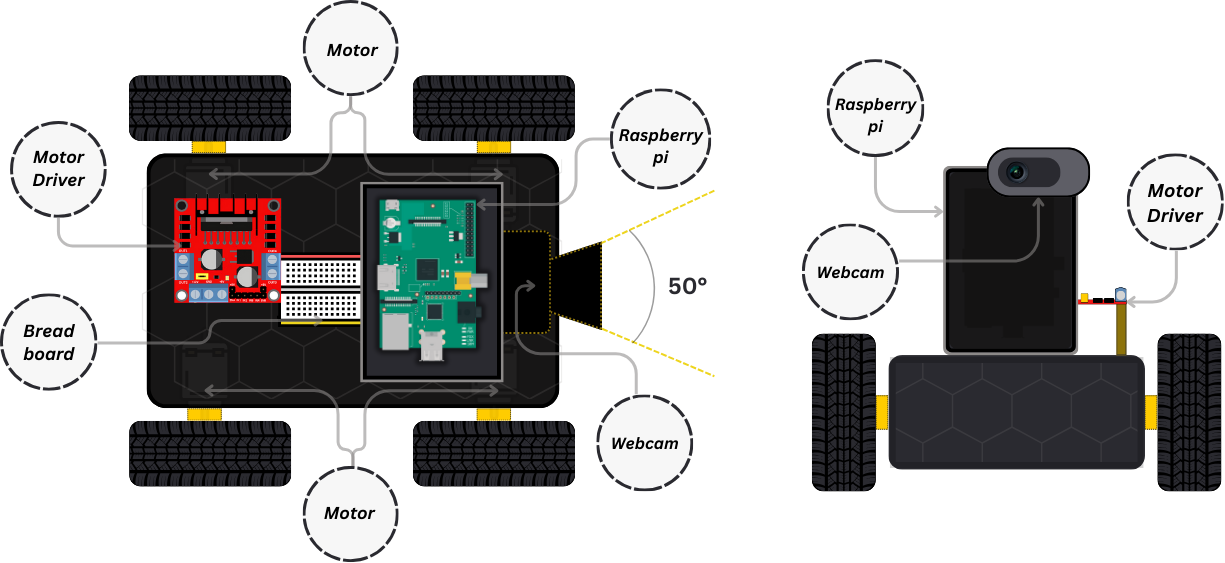
\includegraphics[width=1\textwidth]{ch4/figs/robot_car.png}
	\caption{Illustration of the hardware layout, showing the arrangement of key components like the Raspberry Pi, motor system, and camera module.}
	\label{fig:hardware_layout}
\end{figure}


\section{\label{sec:hardware} Hardware System Architecture}

The system architecture provides a high-level overview of how the robot and its subsystems interact with one another to achieve semi-autonomous navigation, real-time feedback, and remote control functionality. The key components of the system include the hardware modules such as the Raspberry Pi, motors, sensors, and camera, alongside software elements such as computer vision algorithms and the web-based control interface.

The project is composed of several key components, below is a high level overview of all the components that are needed in order execute the project properly.

\section{Microcontroller Selection}

The Raspberry Pi Model 4B with 4GB RAM was selected as the microcontroller for this project due to its versatility and capability to handle multiple complex tasks simultaneously. Its ability to run sophisticated computer vision algorithms while interfacing with other hardware components makes it ideal for this application. The capacity to manage real-time video streaming, marker detection, and motor control simultaneously is crucial for the system's functionality.

Unlike dedicated micro-controllers such as Arduino, the Raspberry Pi can run Python-based frameworks like OpenCV, which is essential for implementing the system's computer vision capabilities. This aligns with findings from Jacobsen et al. \cite{jacobsen2018}, who demonstrated the effectiveness of using a Raspberry Pi for web hosting.

The use of a single, integrated system for both processing and control, as highlighted in Chapter\ref{ch:lit_review}, simplifies the overall design, reduces latency, and enhances system performance. In our setup, the Raspberry Pi functions as the central processing unit, responsible for interfacing with all other components. It processes the video feed from the camera, executes computer vision algorithms such as ArUco marker detection, and transmits control signals to the motor driver. The Raspberry Pi runs a Python-based framework that integrates OpenCV for vision tasks and SocketIO for communication with the web interface. This allows it to receive input from the camera, process it using OpenCV, and then send commands to the motor driver based on the detected environment and user instructions received through the control interface.

The selection of the 4GB RAM version was made to ensure sufficient memory for running multiple processes concurrently and handling intensive computational tasks. While the 8GB version offers more memory, the 4GB model provides a balanced compromise between performance and cost-effectiveness for our application. Table \ref{table:pi_specs} provides a comparison of the specifications for the Raspberry Pi Model 4B with 4GB RAM:


\begin{table}[h!]
	\centering
	\begin{tabular}{|l|c|c|c|}
		\hline
		\textbf{Specification} & \textbf{2GB RAM} & \textbf{4GB RAM} & \textbf{8GB RAM} \\
		\hline
		\textbf{CPU} & Quad-core Cortex-A72 & Quad-core Cortex-A72 & Quad-core Cortex-A72 \\
		\hline
		\textbf{Clock Speed} & 1.5 GHz & 1.5 GHz & 1.5 GHz \\
		\hline
		\textbf{RAM} & 2GB LPDDR4 & 4GB LPDDR4 & 8GB LPDDR4 \\
		\hline
		\textbf{Networking} & Gigabit Ethernet & Gigabit Ethernet & Gigabit Ethernet \\
		\hline
		\textbf{USB Ports} & 2x USB 3.0, 2x USB 2.0 & 2x USB 3.0, 2x USB 2.0 & 2x USB 3.0, 2x USB 2.0 \\
		\hline
		\textbf{Video Output} & 2x micro-HDMI & 2x micro-HDMI & 2x micro-HDMI \\
		\hline
		\textbf{Power Supply} & 5V/3A USB-C & 5V/3A USB-C & 5V/3A USB-C \\
		\hline
	\end{tabular}
	\caption{Comparison of Raspberry Pi Model 4B RAM Versions}
	\label{table:pi_specs}
\end{table}

This hardware configuration provides the necessary processing power and memory to handle the computer vision tasks, video streaming, and robot control required by our project. The Raspberry Pi 4B with 4GB RAM offers a robust platform capable of running complex algorithms, processing real-time video data, and managing the various input and output operations essential for the robot car's operation.

\subsection{Camera Module}
The camera plays a pivotal role in this system as it provides real-time feedback necessary for detecting fiducial markers and controlling the robot's movement. The decision to use a high-resolution web camera, specifically the HD Logitech C270, over a more basic sensor was based on the need for precise marker detection, which demands high-quality image capture. La Delfa et al. \cite{delfa2015} emphasized the importance of high-resolution cameras for accurate marker detection, particularly in dynamic environments. A higher-quality video feed improves the reliability of computer vision algorithms and ensures better control over the robot’s movements.

The camera module continuously captures the video feed, which is streamed to both the user via the web interface and the Raspberry Pi for processing. The camera plays a critical role in detecting fiducial markers in the environment, enabling navigation and interaction based on visual feedback.

\begin{table}[h!]
	\centering
	\caption{Comparison between Logitech C270 and Raspberry Pi Camera Module}
	\begin{tabular}{|p{4cm}|>{\centering\arraybackslash}p{5cm}|>{\centering\arraybackslash}p{5cm}|}
		\hline
		\textbf{Specification} & \textbf{Logitech C270}               & \textbf{Raspberry Pi Camera Module V2} \\ \hline
		Resolution             & 1280x720 (HD)                        & 3280x2464 (8 MP)                       \\ \hline
		Frame Rate             & 30 fps (at 720p)                     & 30 fps (at 1080p)                      \\ \hline
		Field of View (FOV)    & 60°                                  & 62.2°                                  \\ \hline
		Interface              & USB                                  & CSI (Camera Serial Interface)          \\ \hline
		Price                  & readily-available                             & Low                                    \\ \hline
		Ease of Use            & Plug-and-play                        & Requires configuration                 \\ \hline
		Compatibility          & Universal (works on various systems) & Raspberry Pi exclusive                 \\ \hline
	\end{tabular}
	\label{tab:camera_comparison}
\end{table}


The Logitech C270 was chosen primarily due to it being readily available for use and its ability to seamlessly integrate into various systems via USB, requiring minimal configuration compared to the Raspberry Pi Camera Module. Additionally, while the Raspberry Pi camera offers higher resolution, the Logitech C270 provides sufficient image quality for marker detection. Furthermore, the webcam is universally compatible, making it a practical choice for prototyping and development in this context.

The camera module continuously captures the video feed, which is streamed to both the user via the web interface and the Raspberry Pi for processing. The camera plays a critical role in detecting fiducial markers in the environment, enabling navigation and interaction based on visual feedback.

\subsection{Motor and Drive System}

The four-wheel drive system of the DGU ALUM MULTI-CHASSIS 4WD KIT was selected to ensure that the robot can move with precision across various terrains. This chassis provides a sturdy foundation for the robot's movement capabilities. The motors used in this system operate on 3V\textasciitilde12VDC, with a maximum torque of 800gf cm MIN at 3V and a no-load speed of 1:48 at 3V. Each motor measures 7x2.2x1.8cm and draws a load current of 70mA (250mA MAX) at 3V. The use of an L298N H-bridge motor driver allows for efficient control of these motors via Pulse Width Modulation (PWM) signals from the Raspberry Pi, enabling fine-grained control over the speed and direction of each motor.

According to Vanitha et al. \cite{vanitha2016}, a robust motor and drive system is essential for mobile robots that rely on real-time feedback from sensors for navigation. The choice of using an H-bridge for motor control is well-supported in robotics literature as it allows for both forward and reverse motion, as well as braking, without adding unnecessary complexity. The four-wheel drive system enables the robot's movement and maneuvering, with the L298N motor driver controlling the speed and direction of the motors based on the PWM signals received from the Raspberry Pi. This setup allows the system to adjust motor power dynamically to maintain proper navigation based on sensor input or user commands, achieving precise movement in various scenarios.

\begin{figure}[H]
	\centering

		\centering
		\includegraphics[width=0.835\textwidth]{ch4/figs/H-Bridge-Interface.png}
		\caption{Illustration of the H-Bridge connection with the motors.}
		\label{fig:motor_H-bridge_connection}
	\end{figure}


\begin{table}[h]
	\centering
	\begin{tabular}{|c|c|c|c|c|c|c|}
		\hline
		\textbf{IN1} & \textbf{IN2} & \textbf{IN3} & \textbf{IN4} & \textbf{Motor A/B} & \textbf{Motor C/D} & \textbf{Robot Movement} \\
		\hline
		0 & 1 & 0 & 1 & Forward & Forward & Forward \\
		\hline
		1 & 0 & 1 & 0 & Reverse & Reverse & Reverse \\
		\hline
		0 & 1 & 1 & 0 & Forward & Reverse & Right Turn \\
		\hline
		1 & 0 & 0 & 1 & Reverse & Forward & Left Turn \\
		\hline
		0 & 0 & 0 & 0 & Stop & Stop & Stop \\
		\hline
		1 & 1 & 1 & 1 & Brake & Brake & Brake \\
		\hline
	\end{tabular}
	\caption{Truth Table for L298N H-Bridge Motor Control}
	\label{tab:condensed_hbridge_control}
\end{table}

The Raspberry Pi generates PWM (Pulse Width Modulation) signals through its GPIO pins, which are connected to the input pins (IN1, IN2, IN3, IN4) of the L298N H-bridge motor driver. These digital signals control the direction and speed of the motors. The H-bridge then interprets these signals and converts them into the appropriate voltage levels and current flow to drive the motors. For Motors A and B, IN1 and IN2 control their direction and speed, while IN3 and IN4 control Motors C and D. The H-bridge acts as an intermediary, amplifying the low-power signals from the Raspberry Pi into the higher power (by using an external power source) needed to drive the DC motors effectively. This setup allows for precise control over each motor's behavior, enabling complex movements of the robot through simple digital commands from the Raspberry Pi.

\section{Power Supply}

Although the primary focus of this project is the robot's navigation, control systems, and augmented reality (AR) integration, the power supply plays a vital role in ensuring reliable performance for the entire system. Without a stable and appropriate power source, the Raspberry Pi, motors, and other components would fail to operate consistently, which could result in unpredictable robot behavior. To address the varying power needs of the system components, two separate power supplies were implemented.

\subsection{Raspberry Pi Power Supply}
The Raspberry Pi requires a consistent and stable power supply to handle its computational tasks, including image processing, web-based control, and communication with other subsystems. A power bank was selected for this purpose due to its wide availability, ease of use, and sufficient power output.

\begin{itemize}
	\item \textbf{Power Source:} A commercial power bank with a 2.1A output was utilized to meet the power requirements of the Raspberry Pi 4.
	
	\item \textbf{Reason for Choice:} The Raspberry Pi 4 requires a power supply that can provide at least \textbf{5V and 3A} for optimal performance. While the chosen power bank offers slightly lower current (2.1A), testing showed that it was sufficient for running the robot's tasks without significant performance degradation. Additionally, the portability and long-lasting capacity of the power bank make it ideal for mobile robotics applications.
	
	\item \textbf{Justification:} Based on several studies on mobile robot systems, power banks are commonly employed due to their flexibility and ability to deliver steady voltage, especially in outdoor or mobile environments. This setup also avoids the need for complex, custom-made power circuits that would otherwise add unnecessary complexity to the system.
\end{itemize}

\subsection{H-Bridge and Motor Power Supply}
The L298N H-bridge motor driver and the motors require a different power supply than the Raspberry Pi, given their higher power demands during operation, particularly under load (e.g., when turning or climbing). To meet this requirement, an RS PRO 3C 3S1P Li-Ion Battery Pack was chosen, which offers higher voltage and capacity.

\begin{itemize}
	\item \textbf{Power Source:} The battery pack consists of \textbf{three 18650 Li-Ion cells} connected in series (3S1P configuration), providing a total voltage of \textbf{11.1V} and a capacity of \textbf{2600mAh}.
	
	\item \textbf{Specifications:}
	\begin{itemize}
		\item Voltage: 11.1V
		\item Capacity: 2600mAh
		\item Configuration: 3 x 18650 cells in series
	\end{itemize}
	
	\item \textbf{Reason for Choice:} The L298N H-bridge can handle up to 46V, so 11.1V is well within its operational range. The motors benefit from higher voltage when performing tasks that require more torque, such as sharp turns or accelerating from a stationary position. The 2600mAh capacity ensures that the robot can operate for extended periods before needing a recharge.
	
	\item \textbf{Justification:} As highlighted in the literature, motor-driven robots require a power supply that can deliver sufficient current and voltage, especially when navigating uneven terrain or performing high-torque tasks like turning. The chosen battery pack is a reliable option for robotics applications because it balances compactness, durability, and energy density.
\end{itemize}

\section{\label{sec:software} Software System Architecture}

The bulk of the project relied on software to function, as it serves as the brain of the entire system, orchestrating the communication between hardware components and enabling real-time decision-making. This architecture integrates several critical subsystems including computer vision, motor control, data processing, and network communication. The primary software components were developed in Python due to its versatility and rich library ecosystem, particularly in robotics, image processing (OpenCV), and web development (Flask).


\begin{figure}[H]
	\centering
	
	\centering
	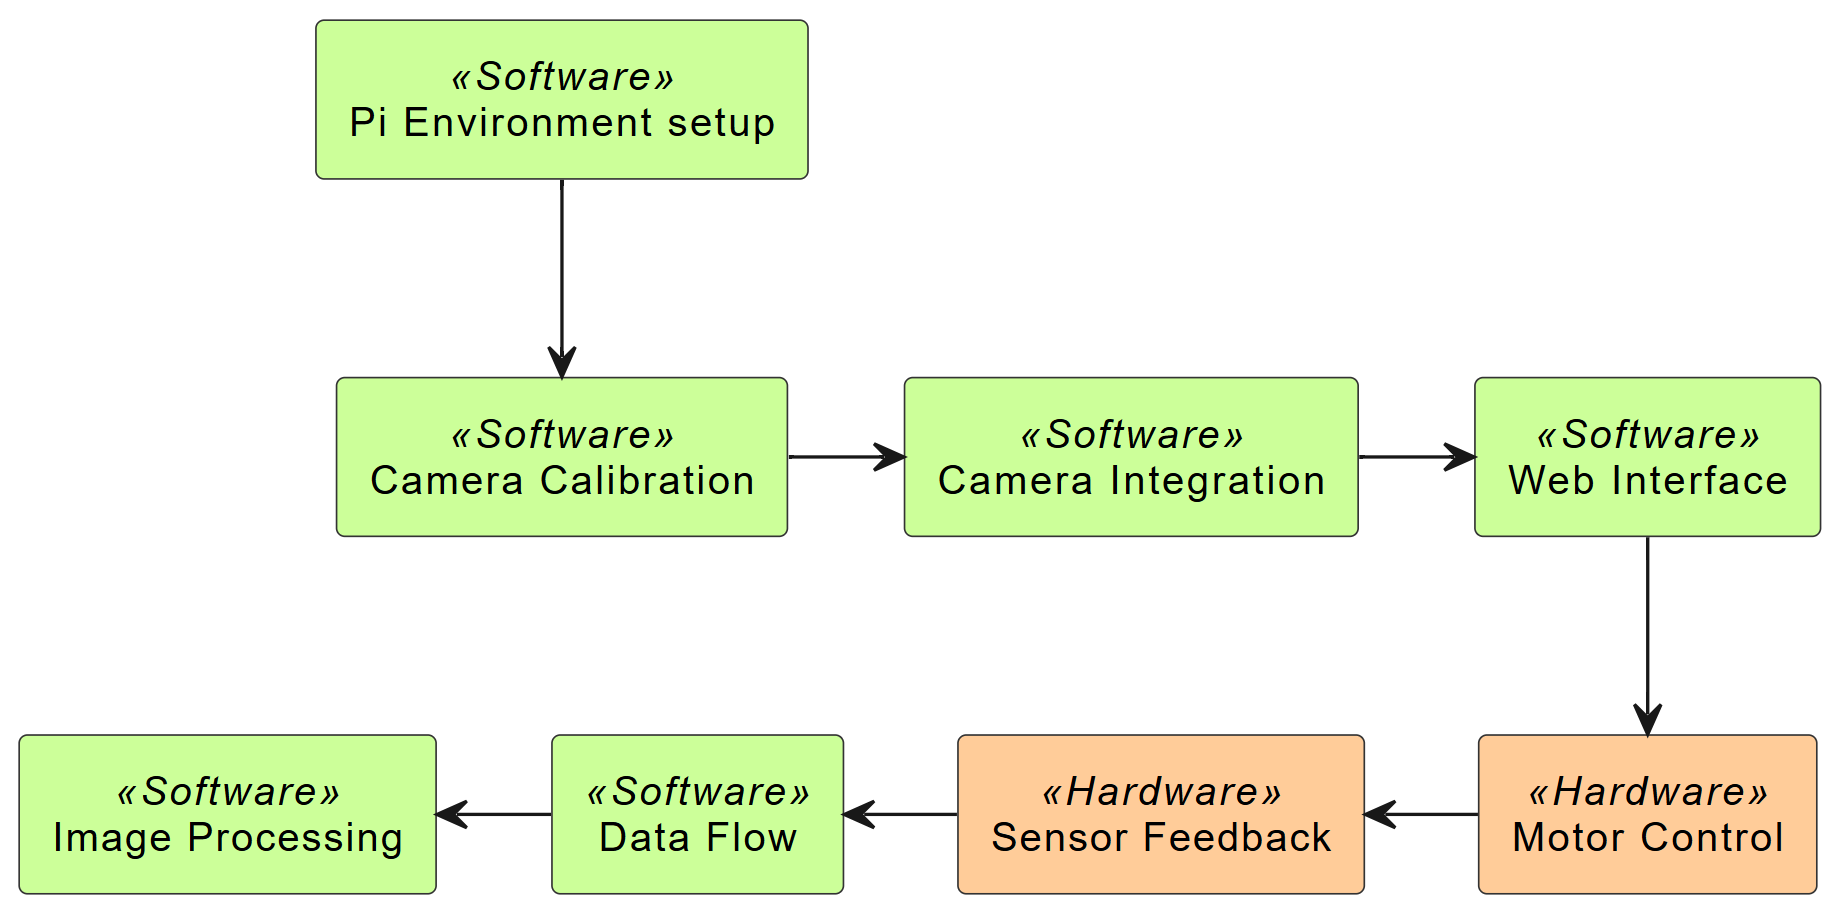
\includegraphics[width=0.8\textwidth]{ch4/figs/hi.png}
	\caption{Illustration of the project production process.}
	\label{fig:moto}
\end{figure}

\subsection{Development Environment Setup}

To begin the development of the robot, I set up a **headless Raspberry Pi** environment, which means that I connected to the Pi remotely over SSH, avoiding the need for a physical monitor, keyboard, or mouse. This headless setup is common for Raspberry Pi projects where the Pi is used as an embedded device, and allows for easier control via the network from my laptop. I initiated an SSH session using the command:

\begin{quote}
	\texttt{ssh pi@<raspberry-pi-ip>}
\end{quote}

from my development machine to connect to the Pi and began the process of setting up the environment.

The primary goal of the development environment was to create a clean, isolated workspace that would avoid interfering with the **Pi’s system libraries** and default configurations. To achieve this, I decided to set up a **virtual Python environment** using \texttt{venv}, which would ensure that all libraries required for this project were contained within the environment and did not alter the system’s default Python packages.

To create and activate the environment, I ran:

\begin{quote}
	\texttt{python3 -m venv robot\_env} \\
	\texttt{source robot\_env/bin/activate}
\end{quote}

This created an isolated environment named \texttt{robot\_env}, and activated it so that all subsequent library installations would be confined to this environment. From here, I proceeded to install the essential libraries required for the project.


The project depended on several libraries for various functions. Some of these libraries were for The project depended on several libraries for various functions. Some of these libraries were for \textbf{web development}, like \textbf{Flask} and \textbf{Flask-SocketIO}, which handled real-time communication between the Raspberry Pi and the web interface. Others were for \textbf{computer vision}, including \textbf{OpenCV} and \textbf{ArUco}, which would handle marker detection and processing of the video feed.


To install the required libraries, I used \texttt{pip} within the activated virtual environment. Here is an  command that I used to install all the necessary dependencies:

\begin{quote}
	\texttt{pip install flask flask-socketio opencv-python}
\end{quote}

Each of these libraries served a specific purpose:
\begin{itemize}
	\item \textbf{Flask}: Used to create the web server that would serve the video feed and receive control commands from the user interface.
	\item \textbf{Flask-SocketIO}: Allowed for real-time communication between the Pi and the web browser, facilitating responsive control of the robot.
	\item \textbf{OpenCV}: Essential for the image processing tasks, including capturing the video feed and detecting ArUco markers used for localization and navigation.
	\item \textbf{aiortc}: This provided support for WebRTC, allowing for the live video streaming of the robot’s camera feed to the user.
	\item \textbf{pigpio}: A library used for controlling GPIO pins with finer control, providing more accurate timing than \texttt{RPi.GPIO}.
	\item \textbf{Numpy}: Required for handling array and matrix operations, useful for image and data processing in OpenCV.
	\item \textbf{uuid} and \textbf{asyncio}: Used for generating unique identifiers and handling asynchronous operations in the code, particularly for real-time communication via WebRTC.
\end{itemize}

These libraries were specifically selected to ensure smooth operation of the robot’s core functions, including image processing, real-time control, and web interaction. By managing the project’s dependencies in an isolated virtual environment, I minimized the risk of conflicts and ensured that the project could be easily reproduced or transferred to another system if necessary.

\subsection{Camera Calibration}

Before proceeding with the implementation of the robot’s image processing pipeline, I first verified that the camera was functioning correctly. This involved ensuring that the Raspberry Pi camera module was properly connected and that the Raspberry Pi could capture live video feeds. Once this basic functionality was confirmed, the next step was to calibrate the camera to account for lens distortion, a crucial step for ensuring accurate marker detection later in the project.

To perform the calibration, I ran a \textbf{Flask web application} that captured and stored images from the camera for the calibration process. The process of camera calibration involves capturing multiple images of a checkerboard pattern at various angles, which allows for the correction of geometric distortions such as barrel distortion in the captured images. Using the images, I applied OpenCV’s camera calibration functionality to compute the intrinsic and distortion parameters of the camera.

The Flask app was set up to continuously stream the live feed from the camera and save frames at regular intervals. Below is a brief overview of the code used to capture images from the camera and store them for calibration:

\begin{figure}[H]
	\centering
	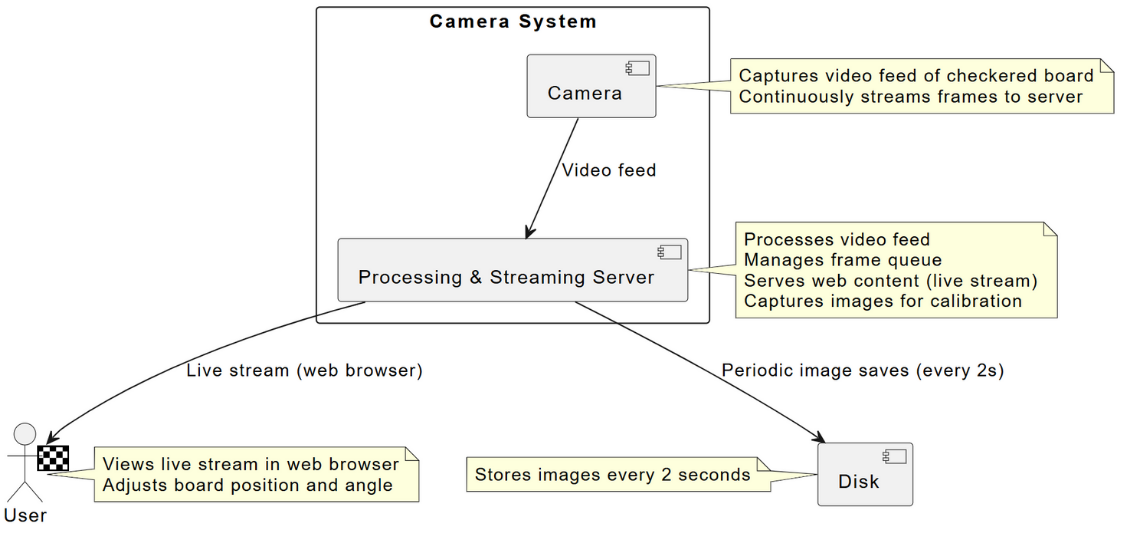
\includegraphics[width=0.9\textwidth]{ch4/figs/calibration.png}
	\caption{Diagram of the functionality of the calibration app.}
	\label{fig:calibration}
\end{figure}

After confirming the camera’s functionality, I captured a series of images through the Flask app, which were then processed using OpenCV’s camera calibration tools. The calibration process computes the intrinsic camera matrix and distortion coefficients, which are essential for removing distortion and ensuring the accuracy of subsequent image processing steps.

OpenCV's camera calibration tool was used, with images of a checkerboard pattern captured by the camera. The following steps were followed for the calibration:

\begin{enumerate}
	\item \textbf{Capture Images}: The Flask app automatically saved images at a regular interval during the video feed, stored in the specified directory.
	\item \textbf{Camera Calibration}: Using OpenCV, the captured images were processed to detect the checkerboard pattern and calculate the camera’s intrinsic and distortion parameters.
	\item \textbf{Saving Results}: Once the camera was successfully calibrated, the calibration parameters (including the camera matrix and distortion coefficients) were saved to a YAML file, which could be used later for distortion correction in real-time video processing.
\end{enumerate}

The resulting calibration file was stored in calibration.yaml, which contained the necessary parameters for correcting lens distortion during subsequent image processing tasks. This YAML file is crucial for ensuring that the robot can accurately interpret the positions of ArUco markers in real-world coordinates, even when captured through distorted lenses.


\subsection{ArUco Marker Detection}


The architecture for ArUco marker detection was designed with the goal of providing accurate and efficient detection of fiducial markers to enhance the robot’s ability to understand and interact with its environment. ArUco markers are widely used in robotics due to their robustness, ease of detection, and the ability to encode unique IDs in each marker, which makes them ideal for navigation, localization, and task execution as already discussed at length in the Literature review.


The detection system is built on top of the OpenCV library, leveraging the \texttt{aruco} module to identify markers in real-time from the camera feed. The architecture includes the following components:

\begin{itemize}
	\item \textbf{Camera Module}: Continuously captures the video stream and sends the frames to the processing unit.
	\item \textbf{Image Preprocessing}: Each frame is first converted to grayscale to reduce computational load and improve detection accuracy. OpenCV’s image filtering tools are used to enhance the quality of the frame and ensure that the markers can be detected even in suboptimal lighting conditions.
	\item \textbf{ArUco Dictionary}: The dictionary is pre-loaded with the specific set of ArUco markers that will be used in the project. This dictionary defines the pattern and structure of the markers to be detected.
	\item \textbf{Marker Detection Algorithm}: The detection algorithm looks for rectangular shapes in the image, computes their corner points, and compares them with the reference markers in the dictionary.
	\item \textbf{Pose Estimation}: Once a marker is detected, its pose (position and orientation) relative to the camera is calculated using the camera's intrinsic parameters, which were obtained from the calibration process.
\end{itemize}

This architecture ensures real-time performance and reliable detection, allowing the robot to respond dynamically to changes in its environment based on the detected markers.


I chose the \textbf{4x4 marker dictionary} for this project because of its balance between detection reliability and encoding capacity. The \texttt{DICT\_4X4\_50} dictionary, which includes 50 unique markers, was particularly suitable for the following reasons:

\begin{itemize}
	\item \textbf{Detection Accuracy}: 4x4 markers are smaller in size compared to larger dictionaries (e.g., 5x5 or 6x6), making them easier to detect at varying distances and angles. Their simplicity reduces computational overhead, which is critical for real-time detection on the Raspberry Pi.
	\item \textbf{Encoding Capacity}: With 50 markers, the dictionary provides enough unique markers to cover a range of tasks, including identifying specific control zones, tracking key landmarks, and providing task-specific instructions. The number of markers is more than sufficient for the scope of this project, which involves interacting with a limited number of known markers.
	\item \textbf{Robustness}: The smaller marker size of 4x4 patterns is more tolerant of slight distortions caused by the camera lens or viewing angle. This makes them ideal for use in dynamic environments where the camera's view of the markers may be imperfect.
	\item \textbf{Efficiency}: Larger dictionaries, such as 5x5 or 6x6, would increase the complexity of detection without providing significant benefits for this specific application. The 4x4 dictionary strikes a balance between detection speed and complexity, making it a more efficient choice for a resource-constrained platform like the Raspberry Pi.
\end{itemize}

\subsection{Web Interface and Server Design}

The design of the web interface and server was a critical component of this project, enabling remote control and real-time monitoring of the robot’s movements. The goal was to create a lightweight and responsive interface that could be accessed through a standard web browser, allowing users to control the robot and view live feedback from the camera in real-time.

\subsubsection{Server Architecture}

The server was built using the Flask framework, a micro web framework for Python, which provides a lightweight yet powerful way to serve dynamic content over HTTP. Flask was chosen for its simplicity and efficiency, making it ideal for handling web requests, streaming video data, and managing control inputs from the user.

The core architecture of the server includes the following key components:
\begin{itemize}
	\item \textbf{Flask Web Server}: Responsible for serving the main web page and handling HTTP requests. Flask's flexibility allows for seamless integration of both static files (e.g., HTML, JavaScript, CSS) and dynamic content (e.g., video streaming).
	\item \textbf{SocketIO Integration}: For real-time communication between the web interface and the robot, Flask-SocketIO was implemented. This allows the web client to send control commands (e.g., movement instructions) to the robot without having to reload the page. SocketIO also enables real-time feedback by pushing notifications and data updates to the client.
	\item \textbf{Video Streaming}: The robot’s camera feed is streamed to the web interface using Flask’s response streaming mechanism. The video is captured frame by frame by the camera, processed, and then sent to the web client, where it is displayed in near real-time.

\end{itemize}

The server continuously listens for incoming client connections, serving the web interface and responding to user inputs. By combining Flask and SocketIO, the system can handle asynchronous events efficiently, ensuring that the robot’s movements are responsive to the user’s input while providing low-latency video feedback.

\subsubsection{Web Interface Design}

The web interface was designed to be intuitive and responsive, allowing the user to control the robot through simple keyboard inputs (W, A, S, D keys) and view a live video stream from the robot’s camera. The interface was built using HTML5, CSS, and JavaScript, ensuring compatibility with modern web browsers.

Key features of the web interface include:
\begin{itemize}
	\item \textbf{Control Panel}: A set of virtual buttons and keyboard inputs for controlling the robot’s movements. These controls are mapped to the robot’s movement functions through SocketIO, ensuring that inputs are transmitted to the robot in real time.
	\item \textbf{Live Video Feed}: A video player embedded in the web page streams the live feed from the robot’s camera. This allows the user to see exactly what the robot sees and make informed control decisions based on the video feed.
	\item \textbf{Feedback and Status Updates}: The interface provides real-time status updates, such as the robot’s current position, speed, and any detected ArUco markers. These updates are pushed to the web client via SocketIO, ensuring the user has continuous feedback on the robot’s status.
\end{itemize}

\subsubsection{Design Considerations}

\textbf{Performance and Latency}: Since the system is designed to operate in real-time, reducing latency in both video streaming and control inputs was a primary concern. Flask-SocketIO was chosen for its ability to handle bi-directional communication efficiently, while the video stream was optimized using a lower resolution and frame rate to reduce the load on the Raspberry Pi and ensure smoother performance.

\textbf{Scalability}: While the system was initially designed for a single user, the architecture allows for future scalability. The use of SocketIO enables multiple clients to connect to the server and receive live updates simultaneously. This could be extended to allow multiple users to observe the robot's movements or control the robot in different contexts.


\subsection{Wheel Interface Design}

The wheel interface was designed to control four motors, arranged in pairs, connected to an L298N H-bridge motor driver. Each pair of motors is responsible for controlling the left and right sides of the robot, allowing for differential steering. The system uses the Raspberry Pi's GPIO pins to control the direction and speed of the motors through Pulse Width Modulation (PWM).

\subsubsection{Motor Control Using GPIO and PWM}

Each motor pair is controlled using two GPIO pins for direction control and one PWM pin for speed control. The L298N H-bridge allows the Raspberry Pi to control the motors in both forward and reverse directions by manipulating the GPIO pins. The PWM signal controls the speed of the motors by adjusting the duty cycle of the signal sent to the H-bridge.

\begin{itemize}
	\item \textbf{Forward Movement}: Both pairs of motors are driven in the same direction, with a high signal sent to the forward GPIO pin and a low signal to the reverse pin. The PWM signal controls the speed of both motor pairs, allowing the robot to move forward.
	\item \textbf{Turning}: To turn, the speed or direction of one pair of motors is adjusted. For example, to turn left, the left motor pair is reversed, while the right motor pair continues to move forward.
	\item \textbf{Stop}: The robot is stopped by setting all GPIO pins to low, cutting off the power to both motor pairs.
\end{itemize}

\subsubsection{Integration with Web Interface}

The web interface allows the user to control the robot in real-time by sending movement commands via Flask-SocketIO. These commands are mapped to motor control functions in the backend, where the GPIO pins are set according to the desired direction and speed. The key inputs (W, A, S, D) correspond to forward, left, backward, and right movements, which are translated into GPIO signals for the motor pairs.

\begin{itemize}
	\item \textbf{W Key}: Moves the robot forward by setting both motor pairs to move in the forward direction.
	\item \textbf{S Key}: Reverses both motor pairs to move the robot backward.
	\item \textbf{A Key}: Adjusts the motor speed and direction to turn left by slowing down or reversing the left motor pair.
	\item \textbf{D Key}: Adjusts the motor speed and direction to turn right by slowing down or reversing the right motor pair.
\end{itemize}

This design provides precise control over the robot’s movements and allows the user to navigate the robot using the web interface in real-time. By using PWM, the robot’s speed can be smoothly adjusted based on the user’s input.

